\section{Annexes}
% par exemple: fragments de code, manuel d'utilisation du logiciel etc


% \begin{thebibliography}{9}
% \bibitem{texbook}
% Donald E. Knuth (1986) \emph{The \TeX{} Book}, Addison-Wesley Professional.

% \bibitem{lamport94}
% Leslie Lamport (1994) \emph{\LaTeX: a document preparation system}, Addison
% Wesley, Massachusetts, 2nd ed.
% \end{thebibliography}
\vspace{0.3cm}
\subsection{Annexe I : Cahier des charges}
\vspace{0.3cm}
\subsubsection*{Objectifs du projet:}
Pour répondre aux attentes de notre projet, nous avons décidé de développer une application web sur laquelle 
nous pourrions jouer au jeu du Hex et de l'Awalé.

Pour chaque jeu nous devons implémenter les règles officielles afin d'assurer une cohérence
entre tous les joueurs. De plus, nous voulons fournir une interface graphique agréable pour l'utilisateur. 
Cela comprend donc une page d'accueil intuitive ainsi que des plateaux de jeu faciles d'utilisation.

\subsubsection*{Description des jeux:}
\begin{itemize}
    \item Hex:
    
    Le Hex est un jeu de stratégie à deux joueurs. Il se compose d'un plateau, de pions bleus
    et de pions rouges. Le plateau du jeu de Hex est composé de cases hexagonales formant un losange. La taille
    du plateau peut varier, mais est généralement de $11\times 11$. Deux côtés opposés du losange sont bleus, les deux 
    autres sont rouges. 

    Le joueur bleu commence. Les joueurs jouent chacun à leur tour. A chaque tour, un joueur place un pion de sa couleur sur une 
    case libre du plateau. Le premier joueur qui réussit à relier ses deux bords par un chemin de pions contigus de sa couleur
    a gagné. Il ne peut y avoir qu'un pion par case. Les pions posés le sont définitivement, ils ne peuvent être ni retirés, ni
    déplacés.\\
    \begin{figure}[h]
        \begin{center}
            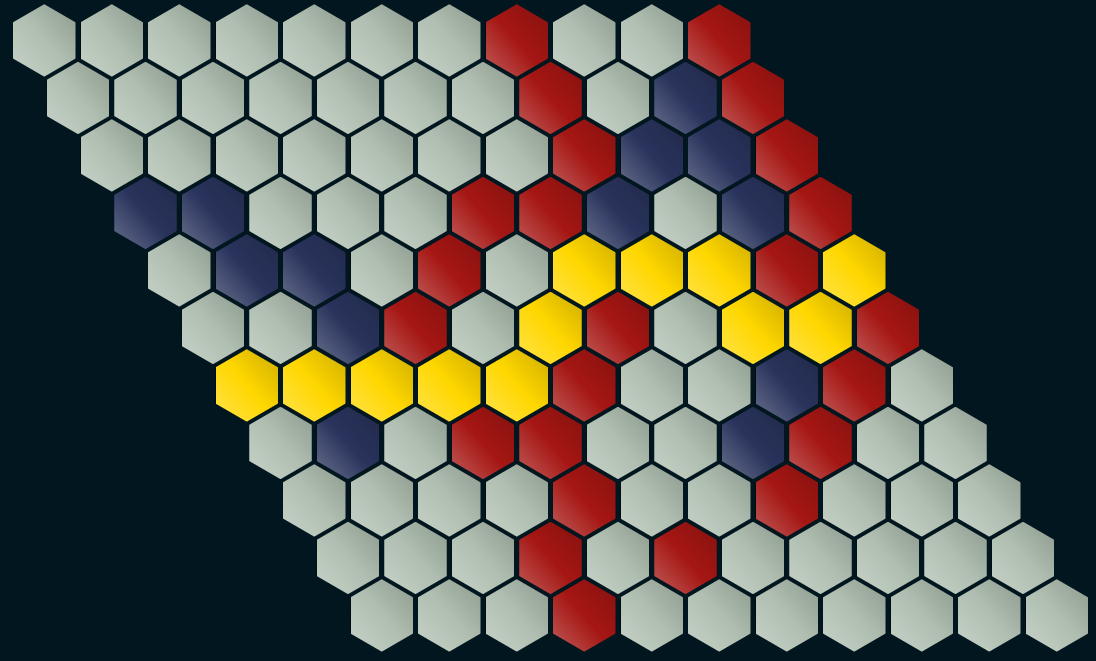
\includegraphics[scale=0.5]{root/hex_jeu_bleu}
        \end{center}
        \caption{Ici bleu a gagné, en reliant ses deux bords.}\label{fig:hex_jeu_bleu}
    \end{figure}
    

    \item Awalé:
    
    L'Awalé est un jeu de stratégie à deux joueurs. Il se compose d'un plateau et de graines. Au début de la partie, 4 graines se 
    situent dans chaque cases du plateau. Les joueurs jouent à tour de rôle. A chaque tour, le joueur prend toutes les graines d’un 
    des trous de son camp puis il les égrène une par une dans toutes les cases qui suivent sur sa rangée puis sur celle de son adversaire 
    suivant le sens de rotation (une graine dans chaque trou après celui où il a récupéré les graines).

    Le joueur « capture » des graines lorsque la dernière case où il pose une graine est une case du camp adversaire et si contient 2 ou 3 
    graines en comptant la nouvelle (elle contenait 1 ou 2 graines avant). Le joueur prend alors les graines de cette case (2 ou 3), puis il 
    prend également les graines de la case précédente si celle-ci répond aux mêmes conditions : être une case du camp adverse et contenir 2 ou 3 graines. 
    Il continue ainsi à prendre les graines des cases antérieures tant que celles-ci répondent aux conditions.

    La première façon qu'une s'achève est lorsqu’un joueur n’a plus de graines dans son camp alors que c’est à lui de jouer et que son adversaire n’est plus en mesure 
    de lui en apporter une selon la règle de « l’obligation de nourrir l’adversaire ». Dans ce cas, son adversaire gagne toutes les graines restantes. C’est 
    la fin par famine.

    La deuxième façon qu'une partie s'achève est lorsqu’il reste trop peu de graines pour qu’aucune prise ne soit désormais possible (en pratique 2 ou 3). 
    Chaque joueur récupère la ou les graines restantes de son camp. C’est la fin par indétermination.
    

\end{itemize}

\subsection*{Fonctionnalités de l'application:}
\begin{itemize}
    \item Possibilité de jouer en joueur contre joueur sur les deux jeux.
    \item Possibilité de jouer en joueur contre IA avec la couleur de notre choix sur  les deux jeux.
    \item Possibilité d'observer une partie entre deux IA sur les deux jeux.
    \item Possibilité d'annuler son dernier coup sur les deux jeux.
    \item Choisir la taille du plateau du Hex. 
    \item Divers boutons pour naviguer à travers l'application.
    \item Possibilité de réinitialiser le plateau des deux jeux lorsqu'on le souhaite.
\end{itemize}

\subsection*{Interface utilisateur:}
L'application s'ouvrira sur une page d'accueil sur laquelle nous pourrons choisir le jeu auquel nous souhaitons jouer.
Pour chaque jeu nous pourrons trouver une page home nous permettant de selectionner le mode de jeu que nous voulons
choisir. Nous retrouverons alors pour les deux jeux les modes joueur contre joueur, joueur contre IA et IA contre IA.

De nombreux boutons de couleur bleus seront mis en place afin de naviguer entre toutes les pages de l'application. D'autres
boutons plus petit seront disponibles. Ils permettront pendant les diverses parties de réinitialiser le plateau de jeu, ou de défaire 
notre dernier coup dans les modes de jeu joueur contre joueur et joueur contre IA.